\chapter{Исследование источника когерентного излучения на основе оптической инжекции на устойчивость к лазерному засеиванию мощным излучением}\label{ch:ch5}
\section{Введение}
На данный момент в практических системах квантового распределения ключей в качестве источника одиночных фотонов используется ослабленный лазерный источник. Это открывает для подслушивающего устройства множество возможностей атаковать источник КРК и получить информацию о секретном ключе. Обычно в качестве контрмеры против атак на источник света КРК рекомендуется использовать некоторую степень изоляции. Однако практические оптические компоненты также могут изменять значение изоляции при внешнем воздействии или под влиянием условий окружающей среды. Здесь мы показываем, что источник на лазерном диоде с внутренним засевом и усилением обладает очень высокой устойчивостью к атакам на внешний лазерный засев, и рекомендуем использовать эту схему в качестве безопасного источника фотонов для систем КРК.
Квантовое распределение ключей (КРК) позволяет двум сторонам генерировать секретный ключ по ненадежному каналу, используя квантово-механические свойства одиночных фотонов. Протоколы КРК в принципе не поддаются взлому. Однако их практическая реализация демонстрирует длинный список побочных каналов, которые могут предоставить подслушивающему лицу дополнительную информацию о секретном ключе и сделать систему, использующую его, небезопасной~\cite{sun2022, makarov2023}. Такие побочные каналы почти всегда являются результатом отличия аппаратного обеспечения от его идеальной модели. 

Одним из наиболее ярких примеров несовершенных устройств являются практические источники фотонов. На сегодняшний день в практических системах КРК используются сильно ослабленные лазерные импульсы от полупроводниковых лазерных диодов (LD), а не истинные однофотонные источники, поскольку последние пока не позволяют достичь практической скорости передачи ключей~\cite{zahidy2024}.
Однако, поскольку полупроводниковые лазеры очень чувствительны к внешним возмущениям, существует несколько атак с лазерной заливкой, которые открывают черные ходы для подслушивающих~\cite{huang2019, pang2020, lovic2023}. Например, предыдущие экспериментальные исследования показали, что мощности инжекции в диапазоне 100 -160 нВт может быть достаточно для управления интенсивностью импульсов Алисы~\cite{huang2019, pang2020}, а мощности даже около 1 нВт может быть достаточно для частичного управления фазой импульсов Алисы~\cite{lovic2023}.

Здесь мы обращаем внимание на то, что описанные выше атаки с лазерным засевом относятся к источнику света, основанному на одном лазерном диоде с усилением. В то же время, LD-источники с инжекционной блокировкой стали широко использоваться в квантовой криптографии, особенно в реализациях квантового распределения ключей, не зависящих от измерительных приборов (MDI КРК)~\cite{wei2020,woodward2021}.

Схема с инжекционной блокировкой источника незаменима для приложений, требующих высокой видимости интерференции между независимыми лазерными источниками. Техника засева света значительно улучшает интерференцию за счет низкого джиттера времени импульса и синхронизации частотных чирпов при сохранении случайных оптических фаз излучаемых лазерных импульсов~\cite{comandar2016a}. Более того, последние исследования показывают, что лазерный источник с внутренним засевом позволяет уменьшить флуктуации интенсивности и тем самым увеличить безопасную скорость передачи ключей при реализации техники decoy-state~\cite{xie2019}. %\AP{add ref}%
 
К сожалению, конфигурация источника с инжекционной блокировкой ранее не тестировалась на устойчивость к атакам с лазерным посевом. Здесь мы впервые исследуем ее оптические характеристики при внешней лазерной атаке с засевом и проводим анализ защищенности при наличии изменений выходного сигнала. Мы показываем, что конфигурация источника фотонов с внутренним засевом является эффективной контрмерой против известных атак на источник фотонов КРК. Между тем, наше исследование демонстрирует и другие эффекты, которые могут иметь место только в исследуемой конфигурации источника. В частности, ведомый лазер действует как ненасыщенный оптический усилитель. Это приводит к независимому усилению сигналов ведущего и Евы и позволяет злоумышленнику извлечь дополнительную информацию о секретном ключе
\begin{figure*}
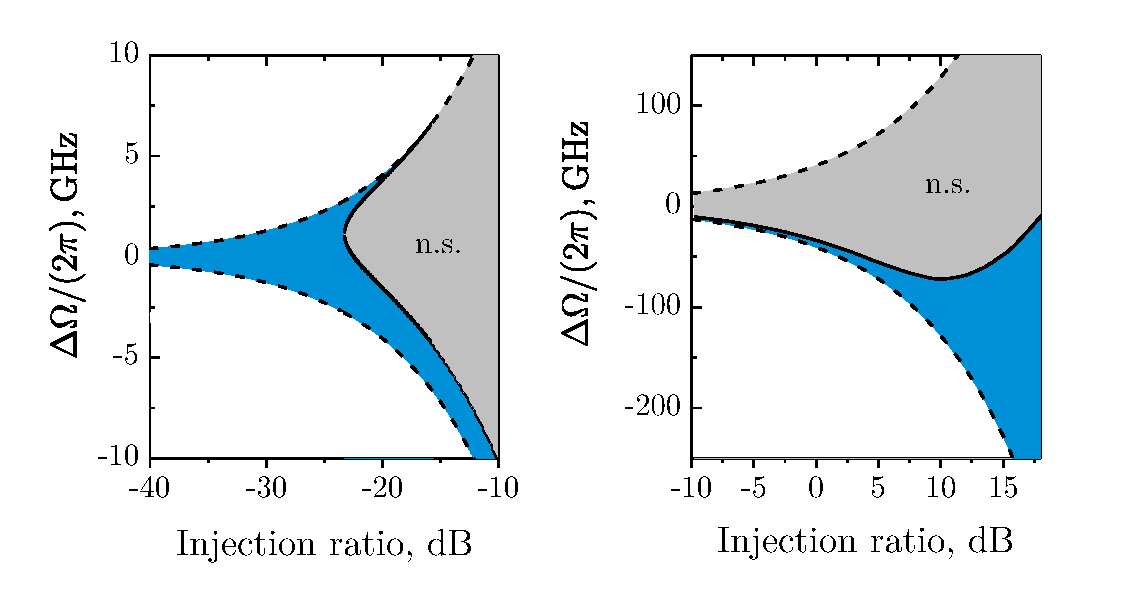
\includegraphics{images/StabilityDiagramsFreq.pdf}
\caption{Locking map versus injection ratio (stable locking is in blue).}
\label{fig:injection_stab ch5}
\end{figure*}
\section{Теоретическое описание метода оптической синхронизации}
\label{sec:theory}

\subsection{Полупроводниковые источники света с инжекционной синхронизацией}

Фазовая синхронизация с помощью оптической инжекции - это метод оптической частотной и фазовой синхронизации, основанный на освещении лазерного резонатора внешним светом. Источник с инжекционной блокировкой содержит "ведущий" лазер, который обеспечивает внешнее излучение для воздействия на "ведомый" лазер~\cite{liu2020}. 

В зависимости от интенсивностей и спектральных показателей ведущего и ведомого ЛД, источник может обеспечивать режим разблокировки, стабильной или нестабильной блокировки~\cite{lau2008}. Эти режимы определяются как области диаграммы с коэффициентом инжекции и частотной подстройкой в виде координат, как показано на \cref{fig:injection_stab}. Частота перестройки - это разность между частотами ведущего и свободно работающего ведомого каналов. Коэффициент инжекции $R_I$ определяется как 

\begin{equation}
\label{eq:injection_coeffitient}
	R_I = -10\times\lg\left({\frac{Q_c^M}{Q_c}} \right),
\end{equation}
%
где $Q_c^M$ и $Q_c$ значения интенсивности ведущего и свободно работающего ведомого лазеров в установившемся режиме, соответственно.
Отметим также, что в импульсном режиме работы ЛД интенсивности $Q_c^M$ и $Q_c$ определяются пиковыми мощностями импульсов как 
\begin{equation}
\label{eq:intens}
	Q = \frac{<P>}{f_R\times\tau_P},
\end{equation}
где $<P>$ - средняя мощность в Ваттах, $f_R$ - частота повторения импульсов, Гц, и $\tau_P$ - длительность импульса, с.
\begin{table}
	\caption{\VM{cite the table in text} Laser parameters used to simulate optical injection.} 
	\label{tab:sim_param}
	\begin{tabular}[t]{@{\extracolsep{1.8ex}}l@{}c@{\quad}l@{}c@{}}
		\hline\hline
		Parameter		&Value  			&Parameter  	& Value	\\ 
		\hline
		$N_{th}$		&$5.5\times10^7$ 	&$N_{tr}$  		& $5.0\times10^7$		\\   
		$\tau_{e}$		&$1~ns$	&$\tau_{ph}$ 	&$1~ps$		\\ 
		$C_{sp}$		&$10^{-5}$ 		& $\Gamma$	& 0.12				\\
		$\alpha$		&5 				& $\kappa_{inj}$	& $5.0\times10^{10} ns^{-1}$	\\  
		I			&$22~mA$	& $\gamma_Q$	& 0				\\
		\hline\hline
	\end{tabular}
	\label{tab:all}
\end{table}
Когда источник работает в режиме стабильной блокировки, ведомый лазер будет вынужден синхронизироваться с ведущим, то есть излучать на той же частоте с фиксированным фазовым смещением. В целом, согласно карте блокировки в \cref{fig:injection_stab}, диапазон блокировки частоты становится больше с увеличением коэффициента инжекции~\cite{wang2013}. Между тем, в практических источниках света для систем QKD коэффициент инжекции отрицательный. Низкий коэффициент инжекции обусловлен двумя факторами. Во-первых, ведомый лазер вносит потери в инжектируемое ведущее излучение. А второй фактор связан с длительностью импульса в соответствии с \cref{eq:intens}. Широко используемый случай реализации оптической схемы предполагает длительность импульса ведомого лазера в несколько раз меньше, чем у ведущего ЛД (в два раза и выше). Это позволяет избежать высокоамплитудных релаксационных осцилляций в выходных импульсах за счет засева ведомого лазера только плоской по интенсивности частью импульсов ведущего. В итоге, для получения высокой стабильности интенсивности исследуемых источников ведущий и свободно работающий ведомый ЛД должны иметь как можно более близкую рабочую длину волны.

\subsection{Многоволновое усиление в полупроводниковых усиливающих средах}

Традиционно полупроводниковые источники с оптической инжекционной блокировкой включают в себя два лазера, ведущий и ведомый лазерные диоды, и теоретически они изучаются в рамках концепции этой конструкции. Однако здесь мы также хотели бы рассмотреть это явление в аспекте усиления излучения в ведомом лазере. Это необходимо для понимания анализа экспериментальных результатов и атак на источник QKD с инжекционной блокировкой. Конструкции волноводов и материал усиления одинаковы или похожи для лазерных диодов и полупроводниковых оптических усилителей (SOA). Разница в том, что в лазерах для генерации и поддержания колебаний вокруг среды усиления формируется резонатор, и сигнал проходит несколько кругов внутри резонатора перед выходом~\cite{chen2022}. Поэтому предположим, что ведомый лазер - это двухпроходной SOA с неидеальным входом, который дает отражения
\subsection{Статистика интерференции фазово-рандомизированного классического света}

Статистические свойства интерференционного сигнала фазово-рандомизированного классического света хорошо изучены и имеют строгие модели, учитывающие все характеристики импульсов~\cite{shakhovoy2020,shakhovoy2021}. Недавно они были разработаны для реализации высококачественных квантовых генераторов случайных сигналов, основанных на интерференции фазово-рандомизированных импульсов. Благодаря этому, используя функцию плотности вероятности интерференционного сигнала, можно дать оценку видимости интерференции, объяснить влияние на нее свойств импульса и, наконец, что очень важно, настроить источник света так, чтобы получить наибольшую видимость интерференции. Поэтому в наших экспериментах мы не измеряем двухфотонную интерференцию, а измеряем и анализируем функцию плотности вероятности интерференции классического света.   

Процедура состоит в следующем. Она включает в себя реализацию несимметричного интерферометра с линией задержки, обеспечивающей время задержки, кратное периоду повторения импульсов. Это приводит к интерференции между импульсами, испускаемыми в разное время. Далее с помощью осциллографа накапливается большая выборка измерений площади интерференционного сигнала и строится гистограмма зависимости числа импульсов от их площади.

В работе~\cite{shakhovoy2021}, авторы показали, что безщелевой колоколообразный лазерный импульс будет иметь двухпиковую форму PDF, где пики будут располагаться на интенсивности конструктивной и деструктивной интерференции, как показано на~\cref{fig:PDF}.
\begin{figure}
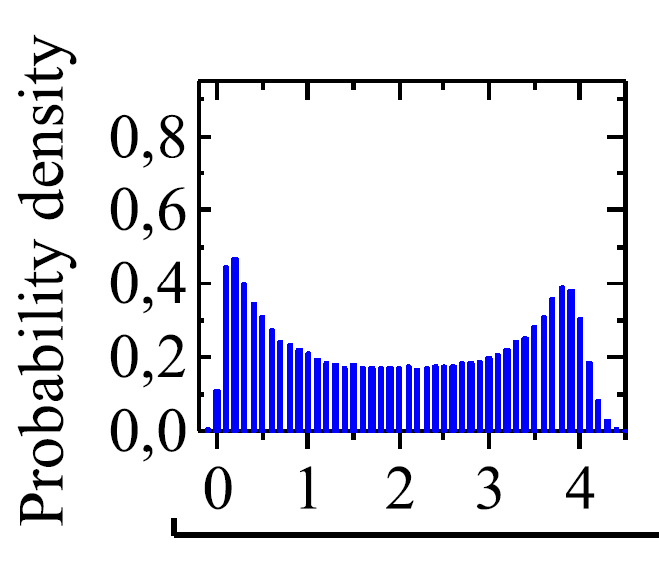
\includegraphics{PDF}
\caption{The PDF of the normalized interference signal of chirpless bell-shaped laser pulse~\cite{shakhovoy2021}.}
\label{fig:PDF}
\end{figure}
Чтобы сравнить ПДФ друг с другом, введем экспериментальную видимость интерференции
\begin{equation}
\label{eq:visibility}
	\eta = {\frac{S_{max} - S_{min}}{4\sqrt{s_1 s_2}}},
\end{equation}
где $S_{max}$ и $S_{min}$ - нормированные интенсивности конструктивной и деструктивной интерференции, определяемые по максимальным экспериментальным вероятностям, $s_1$ и $s_2$ - интенсивности начальных импульсов, которые принимаются равными 1.
\section{Проведение эксперимента}
\label{sec:experiment} 

На риснуке \Cref{fig:setup} показана экспериментальная установка. Она включает в себя три основные части. Это источник света Алисы, подслушивающий семенной лазер и измерительное оборудование. Сначала мы опишем схему источника света, а затем посевной и измерительный конфигурации экспериментальной установки. 
\begin{figure}
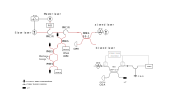
\includegraphics{setup}
\caption{Экспериментальная установка (PM-волокна выделены красным цветом): VOA - переменный оптический аттенюатор, BS - делитель луча, PMCIR - поляризационно-поддерживающий циркулятор, PMBS - поляризационно-поддерживающий делитель луча, PG - генератор импульсов, OPM - измеритель оптической мощности, OSC - осциллограф, OSA - оптический анализатор спектра, BS - делитель луча, LT - световая ловушка, FM - зеркало Фарадея. Коэффициент связи светоделителя (BS) обозначается 99 =: 1× означает, что $99\%$ света проходит в порт, горизонтально противоположный графическому обозначению БС, в то время как $1\%$ света
свет попадает в другой порт}.
\label{fig:setup}
\end{figure}
\subsection{Источник света на испытаниях}

Мы реализовали оптический источник света с инжекционной блокировкой. Его оптическая схема обозначена как Alice в \cref{fig:setup}. Здесь ведущий лазер излучает фазово-рандомизированные импульсы. Они поступают в ведомый лазер через волоконно-оптический циркулятор PMCIR1 (PMCIR-3-A-1550-900-5-08-FA, Optel) из порта~1 в порт~2 и ``засевают'' ведомый лазер. Далее импульсы от ведомого ЛД передаются из порта~2 циркулятора на выход Алисы - порт~3 циркулятора.

В качестве источника мы использовали пару идентичных поляризационно-поддерживающих волоконно-оптических DFB лазерных диодов (Agilecom, WSLS-934010C4124). Они отличаются только наличием встроенного изолятора. У ведущего лазера он есть, а у ведомого - нет. Чтобы избежать нежелательной обратной связи в ведущем лазере с ведомым, ведущий ЛД дополнительно защищен с помощью внешнего волоконно-оптического изолятора (с изоляцией около 60 дБ, не показан в~\cref{fig:setup}). Отметим, что PMCIR1 также обеспечивает изоляцию порта~2 от порта~1 более чем на 40 дБ. В сумме, с учетом типичной изоляции встроенного изолятора около 30 дБ, ведущий лазер изолирован от ведомого лазера более чем на 130 дБ.
 
ЛД питаются при практически нулевом токе смещения от лабораторного источника питания (E3648A, Keysight) с напряжением смещения около 1.2-1.4 В. \AP{Максим, пожалуйста, исправьте это предложение. Я не знаю, как сказать. И дополнительно - об обратном импульсном напряжении}. Для получения оптических импульсов с частотой повторения 10.035 МГц ведущий и ведомый лазерные диоды управляются по отдельности двумя цифровыми генераторами задержки и импульсов (P400, Highland Technology). Электрические импульсы имеют форму квадратной волны и ширину 2.7 нс и 1.9 нс  для управления ведущим и ведомым лазерами, соответственно. Для идеальной формы импульса время прихода ведущего импульса на ведомый диод должно быть немного раньше, чем электрический импульс привода ведомого. Такое согласование времени было достигнуто точной настройкой времени задержки между ПГ с разрешением задержки 1 пс. Время задержки для ведомого лазера составило 7.6 нс
\begin{figure*}
\begin{subfigure}{0.49\linewidth}
	\centering
	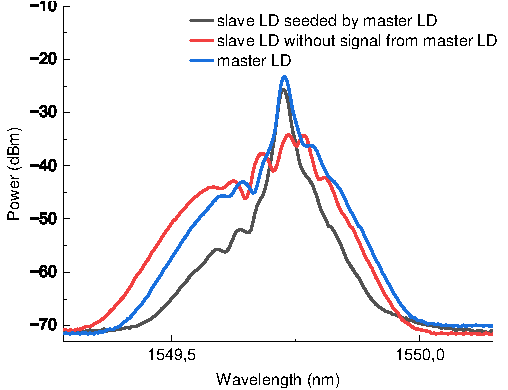
\includegraphics{spectra}
	\caption{}
\end{subfigure}
\hfill
\begin{subfigure}{0.49\linewidth}
	\centering
	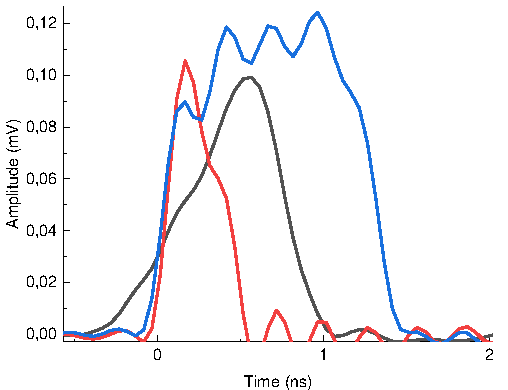
\includegraphics{envelope}
	\caption{}
\end{subfigure}
\caption{Spectral characteristics~(a) and pulse envelope~(b) of the master, slave LDs, and adjusted QKD source. \AP{Here, we saved the pulse shapes using triggering by pulse intensity, in result, we cannot show the delay between master and slave lasers, we might do it manually but seems it is not correct.}}
\label{fig:QKD_source}
\end{figure*}
Здесь мы достигаем согласования спектральных характеристик ведущего и ведомого лазеров путем температурного поворота ЛД с помощью встроенных термоэлектрических охладителей. Фактическая частота отстройки, определяемая как разница между пиковыми частотами ведущего и свободно работающего ведомого, составляет менее 6 ГГц. \Cref{fig:QKD_source} показывает спектральные характеристики и огибающую импульса ведущего ЛД, свободно работающего ведомого ЛД (без сигнала от ведущего ЛД) и всего источника света (ведомый ЛД, засеянный ведущим ЛД) после настройки. 

Максимальная средняя мощность ведущего лазера на входе в ведомый ЛД составляет 11 мкВт. Чтобы избежать изменения спектральных характеристик при изменении мощности ведущего лазера, она изменяется с помощью микроэлектромеханического переменного оптического аттенюатора VOA (V1550PA, Thorlabs). Управляющее напряжение VOA от 0 до $5~\volt$ контролирует затухание, которое может быть увеличено до $25~\deci\bel$ с помощью напряжения. 

\subsection{Экспериментальная установка}

Наша экспериментальная установка моделирует сценарий, в котором Ева атакует источник QKD из квантового канала. Из-за наличия волоконно-оптического циркулятора в схеме источника Алисы, свет подслушивающего устройства может воздействовать только на ведомый лазер; типичная конструкция волоконно-оптического циркулятора не позволяет свету передаваться от порта~3 циркулятора к порту~1.\AP{add ref}

В качестве начального лазера злоумышленника мы использовали лазерный диод с распределенной обратной связью (Gooch and Housego AA1406), усиленный волоконным усилителем на основе легированного эрбием и иттербием волокна (EDFA, заказной блок QGLex)\cite{huang2020}. Он работает в режиме непрерывных волн на рабочей длине волны в диапазоне от 1548.6  до 1550.6 нм, регулируемом регулятором температуры DFB. Применяемая в экспериментах мощность составляет около 500 мВт, поскольку дальнейшее увеличение мощности приводит к изменению вносимых потерь и изоляции циркулятора Алисы PMCIR1. Установка Eve также оснащена делителем луча 99:1 и мониторным измерителем оптической мощности, позволяющим измерять мощность Eve в режиме онлайн. Механический регулятор поляризации установлен для достижения минимальных потерь для света злоумышленника в установке. Свет злоумышленника поступает в источник Алисы через поддерживающий поляризацию волоконно-оптический циркулятор PMCIR2 (PMCIR-3-A-1550-900-5-08-FA, Optel). Далее, прежде чем попасть на целевой ведомый лазер, он проходит в обратном направлении циркулятора Алисы PMCIR1, что обеспечивает изоляцию для света злоумышленника примерно в 46-51 дБ . В результате мощность атакующего лазера, достигающая ведомого лазера Алисы, составляет около 1.8 мкВт .

Конфигурация измерений позволяет контролировать среднюю мощность, спектральные, амплитудно-временные характеристики импульсов и интерференцию следующих друг за другом импульсов. Средняя мощность измеряется с помощью оптического измерителя мощности OPM (S154C, Thorlabs). Выходные спектры измеряются оптическим анализатором спектра OSA (AQ6370D, Yokogawa) со спектральным разрешением 0.02 нм. Амплитуда, длительность импульсов, их стабильность и интерференционные сигналы измеряются осциллографами OSC1 и OSC2 (735Zi, Lecroy, полоса пропускания 3.5 ГГц) и p-i-n фотодиодами (PDI35-10G, Thorlabs) с полосой пропускания 10 ГГц. Для анализа статистических распределений амплитуды и длительности оптических импульсов для каждого измерения накапливается 30 тыс. выборок и строится стандартное отклонение. Затем из средних значений амплитуды и длительности и их стандартных отклонений рассчитываются энергия импульса и его стабильность соответственно.
\begin{figure*}
\begin{subfigure}{0.49\linewidth}
	\centering
	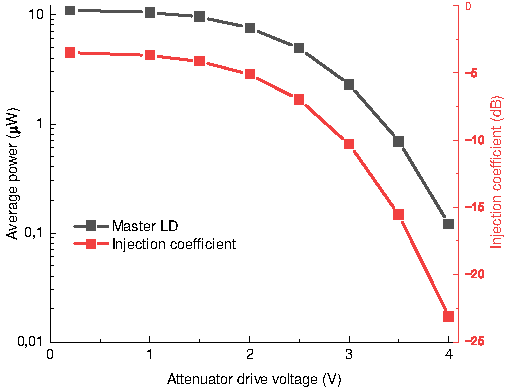
\includegraphics[width=\textwidth]{images/master_power.pdf}
	\caption{}
\end{subfigure}
\hfill
\begin{subfigure}{0.49\linewidth}
	\centering
	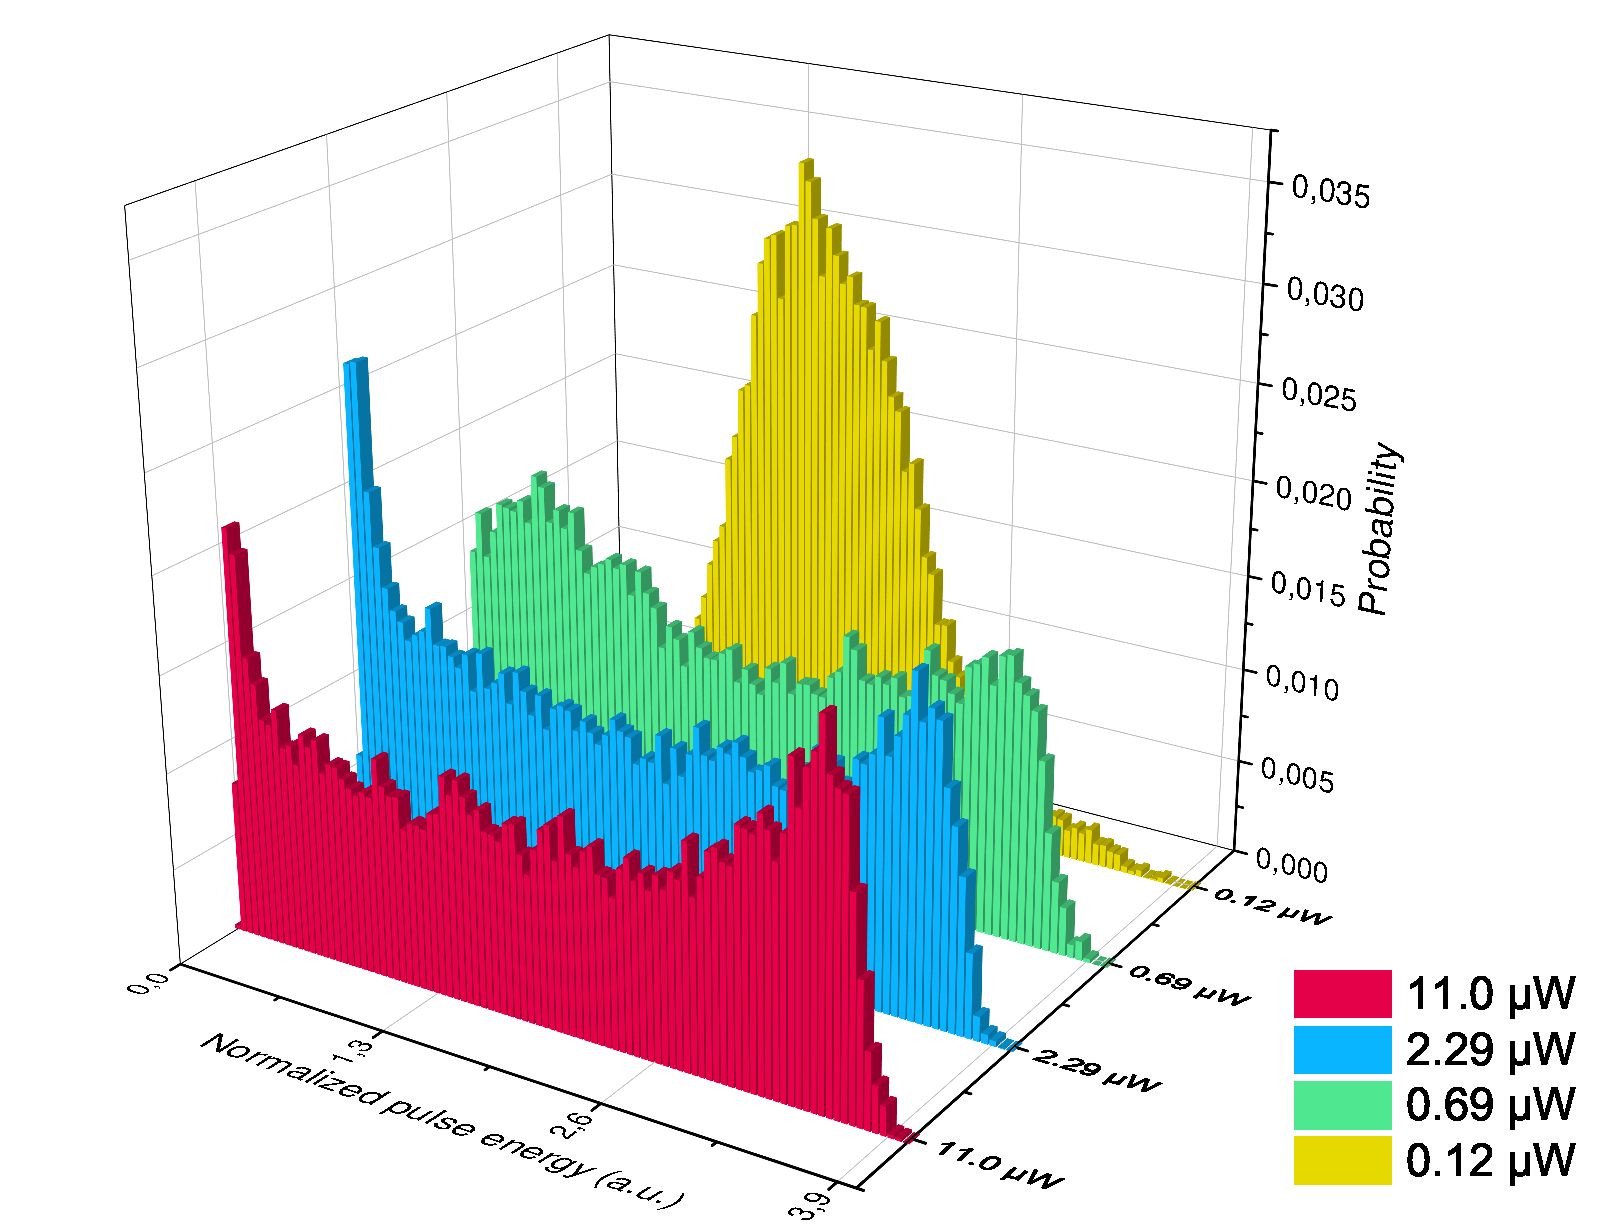
\includegraphics[width=\textwidth]{images/hist_initial.pdf}
	\caption{}
\end{subfigure}
\begin{subfigure}{0.49\linewidth}
	\centering
	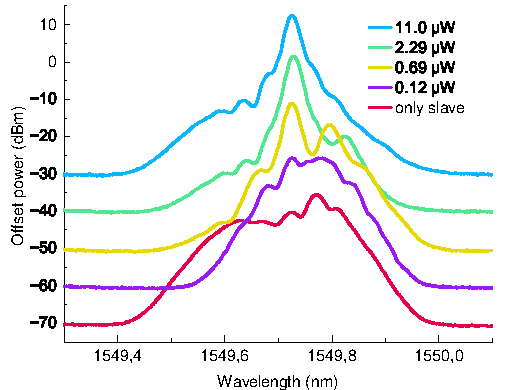
\includegraphics[width=\textwidth]{images/spectra_att.pdf}
	\caption{}
\end{subfigure}
\hfill
\begin{subfigure}{0.49\linewidth}
	\centering
	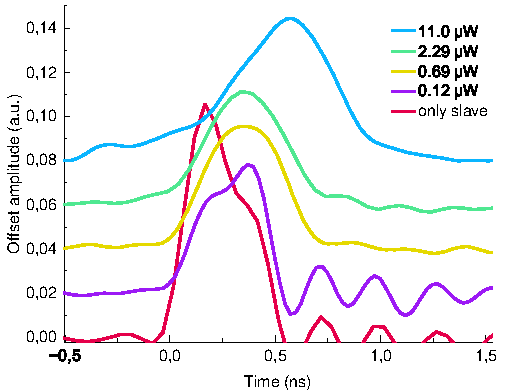
\includegraphics[width=\textwidth]{images/envelope_att.pdf}
	\caption{}
\end{subfigure}
\caption{Характеристики источника QKD в зависимости от напряжения на аттенюаторе: средняя мощность ведущего волокна на входе ведомого волокна (PMCIR1, порт~2) и коэффициент инжекции (a), функция плотности вероятности сигнала помехи (b), выходные спектры (c) и огибающая импульса (d).}
\label{fig:QKD_att}
\end{figure*}
В наших экспериментах мы анализируем качество импульсов, основываясь на форме функции плотности вероятности интерференционного сигнала, как это описано в \cref{sec:theory}C. Чтобы обеспечить интерференцию между следующими друг за другом импульсами, мы реализуем всеволоконный интерферометр Майкельсона на зеркалах Фарадея с линией задержки длиной около 10 метров. Затем, 20 тысяч  измерений площади интерференционного сигнала накапливаются в фиксированном временном интервале (синхронизированном электрическим сигналом тока LD) для построения гистограммы с помощью встроенного осциллографа.

Во-первых, мы полностью охарактеризовали источник QKD для различных мощностей ведущего LD и экспериментально определили границы мощности ведущего LD, необходимые для стабильной оптической инжекции. Далее мы провели серию экспериментов по внешней лазерной атаке на Алису и получили зависимости всех характеристик QKD-источника от средней мощности ведущего ЛД. И, наконец, мы исследовали выходные спектры QKD под воздействием внешнего излучения с различной рабочей длиной волны.
\section{Результаты экспериментов}
\label{sec:results}

\subsection{Характеристики источника QKD}

\Cref{fig:QKD_att} иллюстрирует характеристики источника QKD в зависимости от напряжения управления аттенюатором.

Средняя мощность ведущего ЛД на втором порту PMCIR1 изменяется от 11 до 0.12 мкВт при увеличении напряжения VOA до 4 вольт. \Cref{fig:QKD_att}a демонстрирует эту зависимость и соответствующий расчетный коэффициент инжекции без учета потерь на сопряжении полупроводникового материала с оптическим волокном внутри ведомого лазера (в зависимости от внутренней конструкции ЛД, он может находиться в диапазоне от 1 до 10 дБ). 

Чтобы определить диапазон, в котором ведомый ЛД блокируется излучением ведущего, мы измерили и проанализировали PDF интерференции следующих друг за другом импульсов, спектральные и время-амплитудные характеристики исходящих импульсов для каждой мощности ведущего ЛД, построенные в \cref{fig:QKD_att}a. ПДФ, измеренные для различных мощностей ведущего ЛД (\cref{fig:QKD_att}b), показывают, что блокировка инжекции происходит, когда мощность ведущего ЛД находится в диапазоне от 2.29 до 11 мкВт.  Форма ПДФ имеет два пика, соответствующих идеальной конструктивной и деструктивной интерференции. При мощности основного LD 0.69 мкВт видимость интерференции ухудшается. И, наконец, при минимальной мощности ведущего 0.12 мкВт, PDF имеет только один высокий пик в центре. Это означает, что ведомый не имеет оптической блокировки от ведущего. Без блокировки временной джиттер импульсов увеличивается, что приводит к увеличению вероятности отсутствия помех.

Из спектров и измерений огибающей импульсов (\cref{fig:QKD_att}c и d) также видно, что ведомый ЛД не блокируется излучением ведущего на 0.12 мкВт. Здесь длина волны выходного сигнала отличается от длины волны ведущего, а также форма выходного импульса далека от идеальной колоколообразной формы, на нее влияют релаксационные осцилляции. В ``граничном'' состоянии при мощности ведущего излучения 0.69 мкВт релаксационные колебания в форме импульса отсутствуют, в то же время его спектр имеет второй интенсивный пик, по частоте отличающийся от частоты ведущего LD.

\subsection{Длина волны источника равна длине волны источника}

Как сказано в \cref{sec:experiment}, в нашем эксперименте свет злоумышленника имеет постоянную мощность, а мы изменяем мощность ведущего. \Cref{fig:average_power} демонстрирует зависимость средней мощности источника QKD от мощности ведущего LD для двух случаев: в присутствии света Евы и без него. Для оценки средней оптической мощности атакуемого источника QKD мы сначала измеряем общую среднюю мощность, а затем вычитаем отраженную мощность Евы, измеренную при выключенном источнике QKD. Мы обнаружили увеличение средней выходной мощности на 6-11\%. Как видно из приведенного графика, монотонной зависимости увеличения мощности от мощности ведущего LD не наблюдается. Увеличение мощности значительно варьируется при малом сигнале ведущего устройства и становится постоянным около 8\% $8~\%$, когда мощность ведущего устройства составляет от 7.57 до 11 мкВт.
\begin{figure}
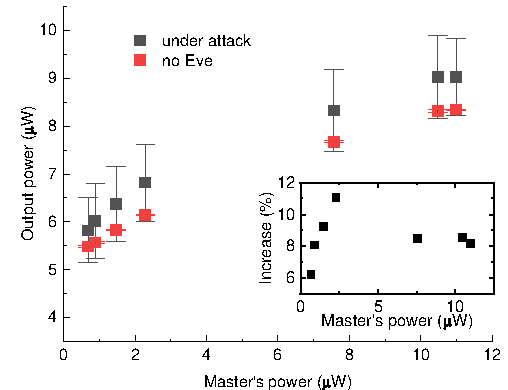
\includegraphics{average_power}
\caption{Средняя выходная мощность источника QKD без Евы и в присутствии атаки с лазерной засечкой.}
\label{fig:average_power}
\end{figure}
Однако более важным является вопрос о том, насколько сильно изменяется энергия импульса. Чтобы ответить на этот вопрос, мы сначала измерили среднюю амплитуду и длительность импульса, а также их стандартное отклонение, рассчитанное на основе выборки размером 30 тысяч. \Cref{fig:area} показывает измеренные амплитуду и длительность, а также рассчитанную нормализованную энергию импульса с атакой и без нее. Из \Cref{fig:area}(a) и (b) видно, что средняя амплитуда импульса увеличивается при атаке, в то время как длительность импульса почти такая же, как и без атаки. Отклонения обеих измеренных величин увеличиваются при атаке. Энергия импульса рассчитывается как умножение измеренной средней амплитуды на среднюю длительность, а стандартное отклонение энергии импульса (SD) - как квадратный корень из суммы квадратов SD измеренных амплитуды и длительности. (Следует отметить, что примененный метод расчета корректен в случае наших экспериментальных данных, поскольку все измеренные формы импульсов имеют однопиковую форму, близкую к колоколообразной, в то время как в общем случае, когда импульсы имеют сложную форму, энергия может перераспределяться между пиками, и, таким образом, площадь импульса должна быть получена из прямых измерений, а не из отдельных измерений амплитуды и длительности импульса). \Cref{fig:area}c показывает энергию импульса с атакой и без атаки, нормированную на энергию без атаки при каждой мощности ведущего ЛД. Вставленный график демонстрирует стандартное отклонение энергии импульса для обоих случаев. Изменение энергии импульса при атаке не показывает зависимости от мощности ведущего LD, она распределяется хаотично. Максимальное увеличение средней энергии импульса составляет 2.8\%$2,8\%$, когда мощность ведущего LD равна 7.57 мкВт. В то же время, колебания энергии импульса увеличиваются во всех исследованных случаях. Стандартное отклонение стало выше примерно на 3\% при атаке по сравнению с результатами без атаки.

Мы также оценили временной джиттер в присутствии и без атаки. Он определяется как стандартное отклонение измерения периода при 30 тыс. отсчетов. Оно составляет 125-128 пс  без света Евы и почти такое же 126-130 пс в присутствии атаки. 
\begin{figure*}
\begin{subfigure}%{0.3\linewidth}
	\centering
	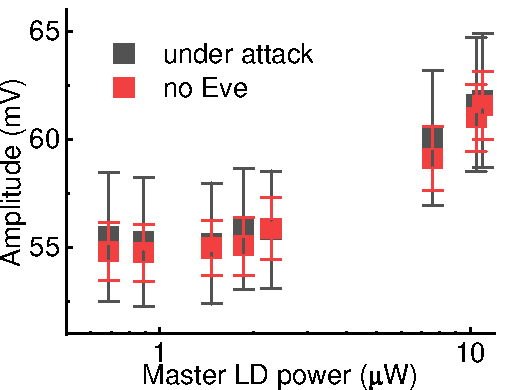
\includegraphics[width=0.4\textwidth]{images/amplitude_change.pdf}
	\caption{}
\end{subfigure}
\hfill
\begin{subfigure}%{0.3\linewidth}
	\centering
	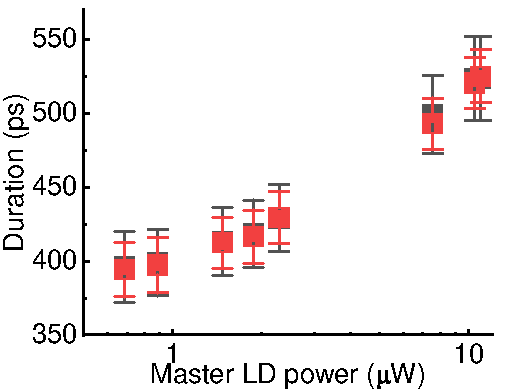
\includegraphics[width=0.4\textwidth]{images/duration_change.pdf}
	\caption{}
\end{subfigure}
\hfill
\begin{subfigure}%{0.3\linewidth}
	\centering
	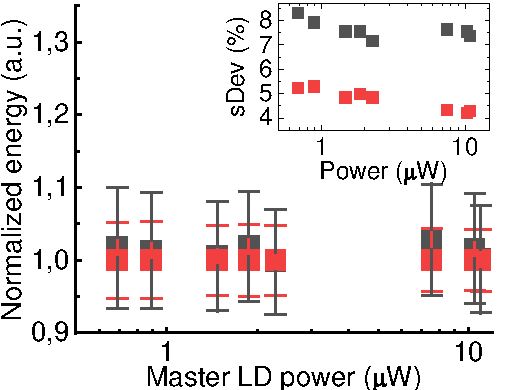
\includegraphics[width=0.4\textwidth]{images/area_under_attack.pdf}
	\caption{}
\end{subfigure}
\caption{Характеристики импульсов с атакой и без: (a)~амплитуда, (b)~длительность и (c)~вычисленная нормализованная энергия импульса (стандартное отклонение указано на вставленном графике).}
\label{fig:area}
\end{figure*}
\begin{figure*}
\begin{subfigure}%{0.49\linewidth}
	\centering
	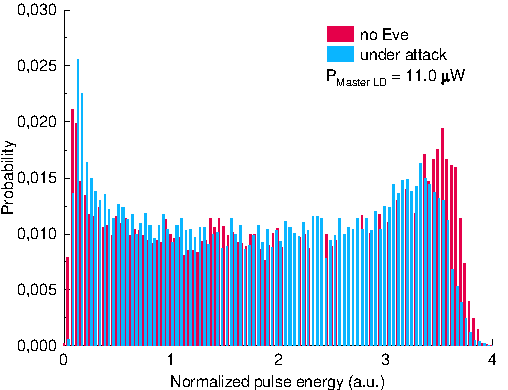
\includegraphics[width=0.75\textwidth]{images/hist_attack_11.pdf}
	\caption{}
\end{subfigure}
\hfill
\begin{subfigure}%{0.49\linewidth}
	\centering
	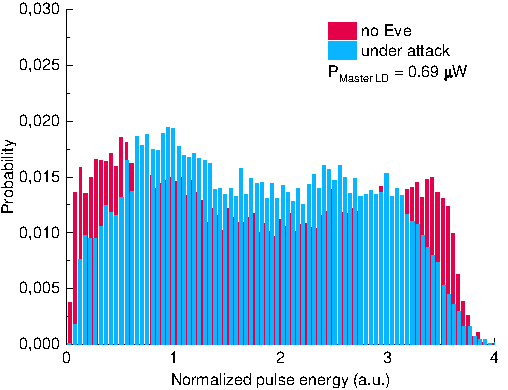
\includegraphics[width=0.75\textwidth]{images/hist_attack_01.pdf}
	\caption{}
\end{subfigure}
\caption{Функция плотности вероятности нормированного сигнала помех с атакой и без нее: (a)~ мощность ведущего LD составляет 11 мкВт; (b)~ мощность ведущего LD составляет 0,69 мкВт.}
\label{fig:histogram}
\end{figure*}
Мы предполагаем, что разница между увеличением средней мощности и энергии импульса означает, что наибольший вклад в увеличение средней мощности вносит усиление излучения Евы в ведомом лазере, а не изменение выходных импульсов. Слабое увеличение энергии импульса и стабильное повышение его стабильности обусловлены слабыми изменениями числа электронов в валентной зоне, вызванными стимулированным поглощением инжектированного света Евы. 

В наших экспериментах мы также количественно оценили влияние инжектированного света на статистику интерференции. \Cref{fig:histogram} позволяет сравнить функции плотности вероятности интерференционного сигнала со светом Евы и без него для двух граничных случаев - когда ведущий лазер принимает максимальное и минимальное значения для обеспечения блокировки инжекции. В обоих случаях мы наблюдаем изменения в PDF из-за атаки внешнего света.

Чтобы количественно оценить влияние света Евы на интерференцию, видимость интерференции оценивается по \cref{eq:visibility}, где ожидаемые интенсивности конструктивной и деструктивной интерференции берутся по пиковым значениям вероятности экспериментальных ПДФ. Видимость уменьшается примерно с 86.4 до 80.1 , когда мощность ведущего устройства принимает максимальное значение в 11 мкВт, примерно с 71.5 до 52.5, когда мощность ведущего устройства составляет 0.69 мкВт . Таким образом, влияние света злоумышленника на интерференционный сигнал усиливается с уменьшением соотношения мощностей хозяина и Евы. Мы предполагаем, что этот эффект вызван смешением усиленного света Евы с мешающими импульсами Алисы и, как было показано в начале текста, увеличением колебаний энергии импульсов, а не фазовой перестройкой между светом ведущего и Евы при его усилении в ведомом ЛД.
\subsection{Атака в зависимости от длины волны}.

Кроме того, мы исследовали влияние начального лазера Евы, работающего на разных длинах волн, на выходной спектр источника QKD. Длина волны атакующего лазера изменялась в зависимости от температуры диода его затравочного лазера, а мощность инжектируемого света Евы была одинаковой во всех измерениях.

\begin{figure}
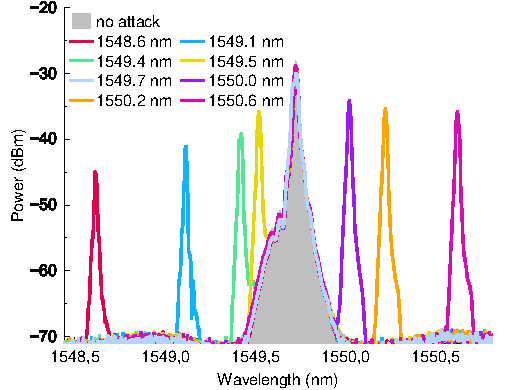
\includegraphics{WL_Eve}
\caption{Спектры выходного сигнала источника QKD для разных длин волн лазера Евы. (Спектры отраженного излучения Евы исключены из измеренных выходных спектров)}.
\label{fig:WL_Eve}
\end{figure}

\Cref{fig:WL_Eve} показывает выходные спектры для различных длин волн затравочного лазера. Спектры атакуемого QKD-источника и отраженного излучения Евы с выключенным QKD-источником измеряются отдельно. Далее, чтобы оценить, усиливает ли ведомый лазер излучение Евы или нет, отраженные спектры вычитаются из спектров атакуемого источника QKD.

Отметим, что реализованная процедура измерения не является точной для получения коэффициентов усиления, более того, спектральное разрешение в 0.02 нм  дает лишь грубую оценку спектральных характеристик при определении характеристик DFB-лазеров. Однако этого достаточно, чтобы показать, что излучение Евы усиливается ведомым лазером в широком спектральном диапазоне.

\section{}